\section{Introduction}
\label{sec:intro}
Businesses and scientists willing to extract knowledge from databases face a
dilemma. On one hand, software editors have commercialized quantity of visual
Business Intelligence tools, such as Tableau or Qlik. Yet, these rely almost
entirely on users' expertise, intuition, and patience. In an exploratory
scenario, when users know little about their data, such tools can involve
time-consuming cycles of trial and error. On the other hand, automated, machine
learning methods have gained much popularity, as shown by the recent success of
industrial ``data scientists''. Nevertheless, at the time of writing this
paper, these experts are still a rare and expensive resource. Can we find a
middle way? Can we design a flexible, accessible method to automatically
analyze data warehouses?

Consider the following scenario. A government analyst studies criminality in US
cities. The database describes how a \emph{measure}, the number of crimes,
varies along several dozen \emph{dimensions}, e.g., the population,
unemployment rate, or location.  Which cities are prone to crime?  Can we
identify causes, correlations, or patterns? For our analyst, inspecting how
every possible combination of dimensions correlates with crime is close to
impossible. But important observations could hide behind unexpected dependencies.
Our aim is to automatically \emph{generate hypotheses} about what influences
the measure.  We want to synthesize SQL queries which highlight what causes
crime to vary, and how these variations occur. Given such queries, even
unexperienced users could explore their data and detect unexpected patterns.

We believe that this problem is extremely common both in business and science,
where multi-dimensional data warehouses have been deployed for years.
Addressing it with an automated method would allow analysts and researchers to
make discoveries more quickly, focusing on interpretation rather than writing
queries. Such a technique could also provoke serendipitous findings, e.g.,
highlighting a surprising correlation or confronting an ill-posed hypothesis.
Besides, the problem is getting more pressing as data warehouses grow in size
and complexity: manual exploration can turn to be out a painful a exercise when
dealing with hundreds of columns.

Automating data exploration is a difficult problem for two reasons.  First, how
do we recognize ``interesting'' queries?  There is, to our knowledge, no
universal measure of inte\-restingness. The challenge is to devise a
theoretically well-founded model, general enough to cover a wide range of use
cases. The second problem is efficiency: given a measure of interest, how can
we explore the space of all database queries quickly enough to support large
datasets? We must design efficient methods to traverse all the possible
combinations of all dimensions.

Several semi-automated exploration frameworks were proposed in the
past, in the context of OLAP data cubes~\cite{sarawagi1998discovery,
imielinski2002cubegrades}. They assumed that databases contained less than a
dozen well-known dimensions.  The whole challenge was to drill-in correctly, in
order to locate ``exceptions'', e.g., local anomalies. We believe that many of
these assumptions do not hold anymore. In our model, databases can contain more
than a hundred dimensions with mixed types. Analysts have little to no
knowledge about the effects of these, even less about their combination.
Therefore, we seek \emph{macro}-deviations: our challenge is to depict a
general picture of how the measure varies across any possible view on the database.

In this paper, we introduce \textit{Claude}, a hypothesis generator for data
warehouses. Claude's aim is to detect interesting views, i.e., interesting
combination of dimensions, and highlight local patterns in these views. We make
three contributions: (1) We devise a model of what makes a view
``interesting'', using simple notions of information theory. (2)~We present
aggressive methods to detect good views in large data\-bases, based on
approximations and greedy search.  (3) We apply our model to real-life
situations, involving either humans (data exploration by subgroup discovery) or
automatic predictors (classification algorithms).

The rest of this paper is organized as follows. Section~\ref{sec:presentation}
gives an overview of our model, which we refine in
Section~\ref{sec:formalization}. Sections~\ref{sec:approximate} describes how
to compute the quality a view, Section~\ref{sec:column} presents our view
detection algorithm, and Section~\ref{sec:detec} introduces how to detect
points of interest. We present our experiments in
Section~\ref{sec:experiments}, related work in Section~\ref{sec:related} and
conclude in Section~\ref{sec:conclusion}.


\section{Problem Formulation}
\label{sec:presentation}
\begin{figure}[t!]
\centering
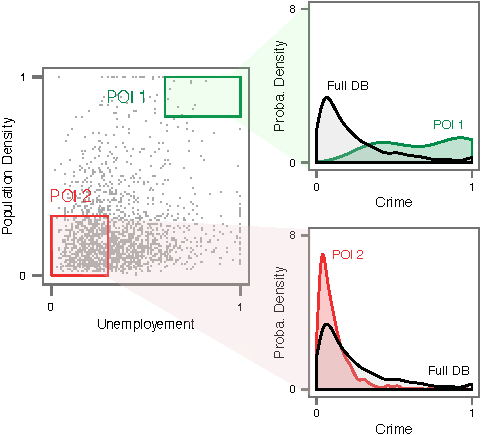
\includegraphics[width=\columnwidth]{images/Overview}
\caption{Example of view, with two points of interest. All the values
are normalized.}
\label{fig:overview}
\end{figure}
Let us define our setting. We reduce our database to a flat table $DB$. This
table contains two types of columns: the \emph{dimensions} $X_0, \ldots, X_N$
and a \emph{measure} (or \emph{target})~$T$. This model is logical, we
are oblivious to the physical structure of the data. Our aim is to describe how
the measure varies across the dimensions. To do so, we want to detect
\textbf{views}, that is, \emph{interesting} selections of dimensions. We also
want to show \emph{why} these views are interesting, by detecting
\textbf{points of interests} (POI). A point of interest is a region in the view
where the measure behaves unusually.

We demonstrate these notions with a running example. We want to understand what
causes crime in US communities. We have a database of cities with several dozen
socio-economic indicators (for instance, employment, age, or diplomas). For
each city we also have the annual number of violent crimes: this is our target
variable. Figure~\ref{fig:overview} presents an example of view. The leftmost
scatterplot pictures the dimensions \texttt{Unemployment} and
\texttt{Population Density}. Why did Claude pick these two columns? The two
POIs provide explanations. Cities with high densities and high unemployment
rates have more crimes (cf. $POI_1$).  Oppositely, cities with low densities
and lower employment rates tend to be safer (cf.  $POI_2$).

In our example, \texttt{Unemployment} and \texttt{Population Density} are
interesting because they influence the target \texttt{Crime}. We can measure
this relationship with statistical dependence. We now introduce the most basic
asumption behind our study: a view is interesting if its dimensions are
\emph{jointly dependent} to the measure. We name this property
\textbf{strength} of a view. From now on we assume that each column $X_n =
(x_n^1, \ldots, x_n^M)$ contains samples from a random variable $\rv{X}_n$, and
that $T$ contains samples from $\rv{T}$.
\begin{definition}
    Consider a view $V = \{X_1, \ldots, X_D\}$, the target $T$, and measure of
    statistical dependence $\mathfrak{S}$. We define the \textbf{strength} of V
    as follows:
    \begin{equation}\label{eq:strengthgen}
        \sigma(V) = \mathfrak{S}(\rv{X}_1, \ldots, \rv{X}_D ; \rv{T})
    \end{equation}
\end{definition}
The statistics literature provides quantity of dependence measures (e.g., the
correlation coefficient). We will introduce our approach
Section~\ref{sec:formalization}.

Observe the two POIs in Figure~\ref{fig:overview}.  The distribution of the
measure \emph{in these regions} differs from its distribution \emph{in the rest
of the database}: it is skewed to the right in $POI_1$, it is skewed to the
left in $POI_2$. In the POIs, the target behaves unusually. We name this
property \textbf{divergence} of the points of interest. We formalize it as
follows. Consider a view based on the random variables $\rv{X}_1, \ldots,
\rv{X}_D$, with respective sample spaces $\Omega_1, \ldots, \Omega_D$.  The set
$R\subset \Omega_1 \times \ldots \times \Omega_D$ represents a region in this
view.  The random variable $\rv{T}$ represents the target \emph{for the whole
database}.  The random variable $\big[ \rv{T} | (\rv{X}_1, \ldots, \rv{X}_D)
\in R \big] $ represents the target \emph{for the tuples within R}. We shorten
this notation to $\rv{T} | R$. The region $R$ is a good point of interest if
$\rv{T} |R $ and $\rv{T}$ have large differences in distribution.
\begin{definition}
    Let $R\subset \Omega_1 \times \ldots \times \Omega_D$ represent a region of 
    the view $\{X_1, \ldots, X_D\}$, and let $\rv{T}$ represent our target
    variable. The function $\mathfrak{D}$ measures the dissimilarity between
    two distributions. We define the \textbf{divergence} of $R$ as follows: 
\begin{equation}\label{eq:divergencegen}
    \delta(R) = \mathfrak{D} \big( \rv{T} | R;  \rv{T}\big)
\end{equation}
\end{definition}
Here again, the statistics literature provides several options to instantiate
$\mathfrak{D}$ (e.g., the difference of the means). We will present our method
in Section~\ref{sec:formalization}.

We are now ready to formulate our problem:
\begin{problem}
Consider a dataset $DB$, a target column $T$, a measure of statistical
dependence $\mathfrak{S}$ and a measure of distribution dissimilarity
$\mathfrak{D}$. Find the top $K$ strongest views with at most $D$ columns. For
each of these views, find the top $P$ divergent POIs.
\end{problem}
To solve this problem, Claude operates in two steps. First, it detects $K$
strong sets of columns.  We call this step \emph{column search}.  Then, it
extracts $P$ POIs for each view. This is the \emph{POI detection} step.

In the rest of this paper, we will illustrate Claude's views with mathematical
notation or visualizations. In reality however, Claude expresses its
recommendations with SQL queries. It returns points of interest as follows:
\begin{verbatim}
    SELECT X1, ... , Xd, T
    FROM DB
    WHERE X1 BETWEEN [L1, H1]
      AND ... 
      AND Xd BETWEEN [Ld, Hd]
\end{verbatim}
In this query, $\texttt{X1},\ldots, \texttt{Xd}$ represent the variables of the
view, $\texttt{[L1, H1]}\ldots\texttt{[Ln, Hn]}$ represents the bounds of the
POI, and $T$ represents the target.




\section{Interestingness Model}
\label{sec:formalization}
We presented views and POIs, but without specifying any measure of dependence
$\mathfrak{S}$ or dissimilarity $\mathfrak{D}$. We now instantiate these
quantities, with elements from information theory.

\subsection{View Strength}
\label{sec:view-strength}
A set of dimensions is interesting if its columns are jointly dependent to the
target. To quantify this dependence, we use the~\emph{mutual information}. This
measure presents many advantages: it is sensible to non-linear dependences, it
can cope with any kind variables, and it is practical to compute. We present it
below.

The \emph{entropy} $H(\rv{X})$ of a variable $\rv{X}$ describes its
variability~\cite{cover2012elements}. If $\rv{X}$ has a constant value, then $H(\rv{X}) = 0$.
Oppositely, if $\rv{X}$ is highly unpredictable (e.g., $\rv{X}$ is
the outcome of flipping a perfectly balanced coin) then $H(\rv{X})$ is
maximal. Formally, if $\rv{X}$ is a discrete variable with sample space
$\Omega$, then we have:
\begin{equation}\label{eq:ent-disc}
    H(\rv{X}) = - \sum_{x\in \Omega} P(\rv{X} = x).\log{P(\rv{X} = x)}
\end{equation}
If $\rv{X}$ is continuous with density $p$, we define it as follows:
\begin{equation}\label{eq:ent-cont}
    H(\rv{X}) = - \int_{-\infty}^{+\infty} p(x).\log{p(x)}\mathrm{d}x
\end{equation}
We can use entropy to describe how variables interact. If two two variables are
dependent, then conditioning (e.g., restricting the range of values) on one
variable will affect the other. In our example, cities with high unemployment
have high levels of crime.  Therefore, conditioning on the variable
\texttt{Unemployment} \emph{decreases the uncertainty} of the variable
\texttt{Crime}. This causes a loss in entropy, and the value of this loss is
the mutual information.  Formally, if $\rv{X}$ and $\rv{T}$ are two
random variables, the expression $H(\rv{T} | \rv{X} = x)$ describes the entropy
of $\rv{T}$ \emph{given $X = x$}. If we average this expression over all
possible values of $x$, we obtain the conditional entropy: $H(\rv{T}|\rv{X}) =
\mathbb{E}_{x} [H(\rv{T} | \rv{X} = x)]$. We define the mutual information $I$
as follows:
\begin{equation}\label{eq:mut-inf}
    I(\rv{X}; \rv{T}) = H(\rv{T}) - H(\rv{T} | \rv{X})
\end{equation}
The mutual information is the loss in entropy between $\rv{T}$ and $\rv{T} |
\rv{X}$. It is symetric, and it is always positive or null. We can generalize
this quantity to joint distributions, which gives us our new, refined version of
view strength:
\begin{equation}\label{eq:strength}
    \sigma(V) = I(\rv{X}_1, \ldots, \rv{X}_D ; \rv{T})
\end{equation}
A view is strong if the mutual information between the target and its
dimensions is high.

In practice, we do not know the distributions of the variables $\rv{X}_n$, but
we have access to the samples $X_n$. Therefore, we \emph{estimate}
the strength. If the variables are discrete, we operates as follow.  We set
$\hat{P}(\rv{X}_n = x) \approx P(\rv{X}_n = x)$ to be the proportion of tuples
with $X_n=x$. We then ``plug'' this estimator in Equations~\ref{eq:ent-disc},
to obtain the estimated entropy $\hat{H}(\rv{X})$. We then use this
approximation in Equation~\ref{eq:mut-inf}.  Dealing with continuous variables
is more difficult, for two reasons. First, estimating the density function in
Equation~\ref{eq:ent-cont} is costly, especially with multivariate
distributions.  Second, it is not clear how to deal with mixed datasets, e.g.
continuous and discrete dimensions, or discrete target and continuous
dimensions.  Therefore, Claude bins all the continuous variables, and treats
them like discrete columns.

\subsection{Points of Interest and Divergence}
Let us now refine our definition of divergence. We established that the
divergence of a POI is the dissimilarity between target's distribution
\emph{within this POI}, and the target's distribution \emph{in the whole
database}.  To measure this dissimilarity, we use the~\emph{Kullback-Leibler
divergence}~(KL).  The KL divergence measures the difference between two
probability distributions. It is null if the two distributions are similar, and
it grows when the distributions differ.  Formally, if $\mathcal{X}$ and
$\mathcal{Y}$ are two discrete random variables with the same sample space
$\Omega$, we have:
\begin{equation}\label{eq:KL_disc} 
    KL\big( \mathcal{X} \parallel \mathcal{Y} \big) = 
    \sum_{x\in \Omega} P(\rv{X} = x).\log{\frac{P(\rv{X} = x)}{P(\rv{Y} = x)}} 
\end{equation}
As Claude discretizes the continuous variables, we ignore the continuous case
(cf.  Section~\ref{sec:view-strength}). Our region $R$ is a good point of
interest if $KL ( \rv{T} |R \parallel \rv{T} )$ is as large as possible:
\begin{equation}\label{eq:divergence}
    \delta(R) = KL \big( \rv{T} | R \parallel \rv{T}\big)
\end{equation}
\begin{figure}[t!]
\centering
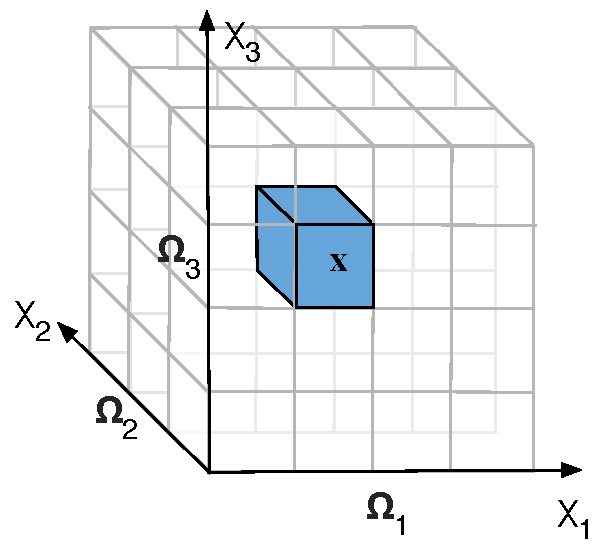
\includegraphics[width=0.4\columnwidth]{images/3Dtest}
\caption{Example of view with three discrete variables $V = \{X_1, X_2, X_3\}$.
The average divergence of the cells $\delta(\mathbf{x})$ equals the strength of
the view  $\sigma(V)$.}
\label{fig:binningexample}
\end{figure}
In fact, view strength and POI divergence are closely related.  Consider a
view $V$.  If $V's$ dimensions are continuous, we bin them. If we compute the
divergence of each tuple and average the results, we obtain the $V$'s strength.
We illustrate this property with Figure~\ref{fig:binningexample}.  Therefore,
strength and divergence are ``two sides of the same coin''. We formalize this
property with the lemma below.
\begin{lemma}
    If $V$ is a view with $d$ discrete variables and $\mathbf{x} \in \Omega_1
    \times \ldots \Omega_D$ is a tuple from this view, then:
    \begin{equation}\label{eq:coin}
        \sigma(V) = \mathbb{E}_{\mathbf{x}}  \big[ \delta(\{\mathbf{x}\}) \big]
    \end{equation}
\end{lemma}
\begin{proof}
    The random vector $\mathbf{X}$ describes a random tuple from $V$.
    Applying Bayes's theorem to Cover and Thomas, Equation
    2.35~\cite{cover2012elements}, we obtain $ I(\mathbf{X} ; \rv{T})
    =\mathbb{E}_{\mathbf{x}}[ KL( T | \{\mathbf{x}\} \parallel T )]$.
    Substituting the left side with Equation~\ref{eq:strength}, and the right
    side with Equation~\ref{eq:divergence}, we obtain the lemma.
\end{proof}
Suppose that we obtained a view $V^*$ by discretizing a set of continuous
variables $V$. The average divergence of the bins equals the strength of $V^*$,
but not that of $V$. Luckily, these quantities converge as the bins get small.
\begin{lemma}
    The view $V$ is a set of continuous variables, $V^b$ is a discretized
    version of $V$ in which each variable is binned with bin size $b$, and
    $\mathbf{x}^b$ is a tuple from $V^b$. We have $\mathbb{E}_{\mathbf{x^b}}
    \big[ \delta(\{\mathbf{x^b}\}) \big] \to  \sigma(V)$ as $b \to 0$.
\end{lemma}
\begin{proof}
    Let the $D$-dimensional random vector $\mathbf{X}$ describe the
    (continuous) variables of $V$, and $\mathbf{X}^b$ describe the (discrete)
    variables of $V^b$. By generalizing Cover and Thomas, Theorem
    8.3.1~\cite{cover2012elements}, we infer that $H(\mathbf{X}^b) + D.\log{b}
    \to H(\mathbf{X})$ as $b \to 0$ .  Thus, using Equation~\ref{eq:mut-inf},
    we have $I(\mathbf{X}^b, \rv{T}) \to I(\mathbf{X}, \rv{T})$. We conclude
    that $\sigma(V^b) \to \sigma(V)$. We apply Equation~\ref{eq:coin} to obtain
    the lemma.
\end{proof}


\section{Approximate View Strength}
\label{sec:approximate}
We now have a formal objective: we want to find the top $K$ views with the
highest strength. At this point, we could easily envision a greedy heuristic to
solve this task. We start with simple views, based on one dimension. We then
add columns, one by one.  To test if a column $X$ is worth adding to a view
$V$, it computes the strength $\sigma(V \cup \{X\})$. If the result is high
enough, we keep the candidate. If not, we discard it. We will indeed present
such an algorithm in Section~\ref{sec:column}. However, we first present a
computational shortcut to obtain $\sigma(V \cup \{X\})$.

We established several ways to compute the strength of a view, with
Equations~\ref{eq:strength} and~\ref{eq:coin}. Nevertheless, none of these
approaches fit incremental algorithms.  Suppose that we wish to compute the
strength of a view $V$, and then the strength of another view $V \cup \{X\}$.
Equations~\ref{eq:strength} and~\ref{eq:coin} give us no opportunity to share
computations.  We must compute $\sigma(V)$ and $\sigma(V \cup \{X\})$
separately. To make things worse, both expressions are expensive, as they
involve group-by queries over the whole database. Therefore, we need to derive
a new \emph{recursive} formulation for the strength of a view:
\begin{lemma}\label{lem:chain}
Consider a view $V = \{X_1, \ldots, X_i\}$, and a target $T$.
For any column $X_{i+1}$: 
\begin{equation}\label{eq:bonus}
    \sigma(V \cup \{X_{i+1}\}) =  \sigma(V) + I(\rv{X}_{i+1} ; \rv{T} | \rv{X}_1 , \ldots, \rv{X}_i)
\end{equation}
\end{lemma}
\begin{proof}
This lemma is a consequence of the Mutual Information's chain rule,
Cover and Thomas, Theorem 2.5.2~\cite{cover2012elements}.
\end{proof}
This lemma describes how adding a column impacts the strength of a view.  For
any random variables $\rv{X}_i, \rv{X}_j, \rv{T}$, the notation
$I(\rv{X}_j;\rv{T}|\rv{X}_i)$  expresses the \emph{conditional mutual
information}. The conditional mutual information is a conditioned version of
the mutual information: it describes the dependency between $\rv{X}_j$ and
$\rv{T}$ \emph{given restrictions on $\rv{X}_i$}. To obtain it, we compute the
mutual information between $\rv{X}_j$ and $\rv{T}$ given all the possible
values of $\rv{X}_i$, and average the results. Formally:
\begin{equation}\label{eq:condmutinfo}
    I(\rv{X}_j;\rv{T}|\rv{X}_i) = \mathbb{E}_{x_i}\big[ I(\rv{X}_j; \rv{T})| \rv{X}_i = x_i)  \big]
\end{equation}
The influence of $\rv{X}_i$ can go either way: it can weaken the dependency between
$\rv{X}_j$ and $\rv{T}$, or it can strengthen it. The conditional mutual information is
positive or null, and it is bounded by the entropy of $\rv{X}_j$ and $T$. 

Unfortunately, we cannot directly exploit Lemma~\ref{lem:chain} in our
algorithm: estimating $I(\rv{X}_{i+1} ; \rv{T} | \rv{X}_1 , \ldots, \rv{X}_i)$
is as expensive as computing $\sigma(V \cup \{X_{i+1}\}) $ directly.  However,
we can use an approximation.  Recall that $V = \{X_1, \ldots, X_i\}$, we
exploit the following observation:
\begin{equation}\label{eq:approx}
\begin{split}
    \sigma(V \cup \{X_{i+1}\}) & = \sigma(V)   + I(\rv{X}_{i+1} ; \rv{T} |
    \rv{X}_1, \ldots, \rv{X}_{i})\\
    & \approx \sigma(V) + I(\rv{X}_{i+1} ; \rv{T} | \rv{X}_{i})
\end{split}
\end{equation}
The idea behind this approximation is naive: we assume that $I(\rv{X}_{i+1} ;
\rv{T} | \rv{X}_1, \ldots, \rv{X}_{i}) \approx I(\rv{X}_{i+1} ; \rv{T} |
\rv{X}_{i})$. We simply ignore the high order dependencies. Thanks to this
assumption, we can compute the strength of our candidates much faster. 

\begin{figure}[t!]
\centering
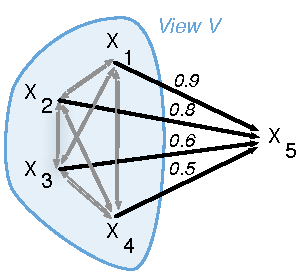
\includegraphics[width=0.4\columnwidth]{images/codependency}
\caption{Example of co-dependency graph with 5 dimensions. To approximate the
strength of $V \cup \{X_5\}$, we add the weight of edge $(X_4, X_5)$ to V's
strength -  in this case 0.5.}
\label{pic:codependency}
\end{figure}
Our new approach operates in two steps, an offline step and an online step.
Offline, we compute the conditional mutual information  $ I(\rv{X}_j ; \rv{T} |
\rv{X}_i)$ between every pair of variable $(\rv{X}_i, \rv{X}_j)$. We call the
resulting structure \textbf{co-dependency graph}. In this graph, the vertices
represent the dimensions, and the edges represent the conditional mutual
information. The co-dependency graph is oriented and weighted.  Online, we run
a greedy algorithm as described previously, but we use Equation~\ref{eq:approx}
to evaluate new candidates.  To compute the strength of a view $V \cup
\{X_{i+1}\}$ with  $V= \{X_1, \ldots, X_i\}$ , we fetch the value of  $
I(\rv{X}_{i+1} ; \rv{T} | \rv{X}_i)$ in the codependency graph and add it to
$V$'s strength. We illustrate this method in Figure~\ref{pic:codependency}.
Previously, computing $\sigma(V \cup \{X_{i+1}\})$ involved heavy groupings and
aggregations on the whole dataset.  Now, we simply perform a lookup in a graph
with $N$ edges, where $N$ is the number of columns in the database.

Our approximation has a drawback: it depends on the order in which we include
the variables in the view. If we enrich a view by successively adding variables
$X_1$, $X_2$ and $X_3$, then we obtain a different strength than if we
incorporate $X_3$, $X_2$ then $X_1$. Similarly, in Equation~\ref{eq:approx}, we
obtain different approximations if we change the indexing of the dimensions
$\rv{X}_1, \ldots, \rv{X}_i$.  For more robustness, we introduce a
``pessimistic'' variant:
\begin{equation}\label{eq:robustapprox}
    \sigma(V \cup \{X_{i+1}\}) 
    \approx \min_{n \in [1, i]} \sigma(V) + I(\rv{X}_{i+1} ; \rv{T} | \rv{X}_{n})
\end{equation}
Instead of adding the strength $I(\rv{X}_{i+1}; \rv{T} | \rv{X}_i)$, where
$\rv{X}_i$ is the last variable inserted, we add $I(\rv{X}_{i+1}; T |
\rv{X}_n)$, where $\rv{X}_n$ is the variable which weakens $\rv{X}_{i+1}$ the
most. We will use this version in the rest of the paper.







\section{Practical Column selection}
\label{sec:column}
This section presents our view search strategy. Our aim is to find the top $K$
views with at most $D$ columns. If our database includes $N$ dimensions, our
search space contains $\sum_{n \leq N} \binom{N}{n} = 2^N$ combinations, which
is clearly impractical. Therefore, we resort to a  greedy, level-wise
heuristic.

\subsection{Base algorithm}
\label{sec:base}
\begin{figure}[t!]
\centering
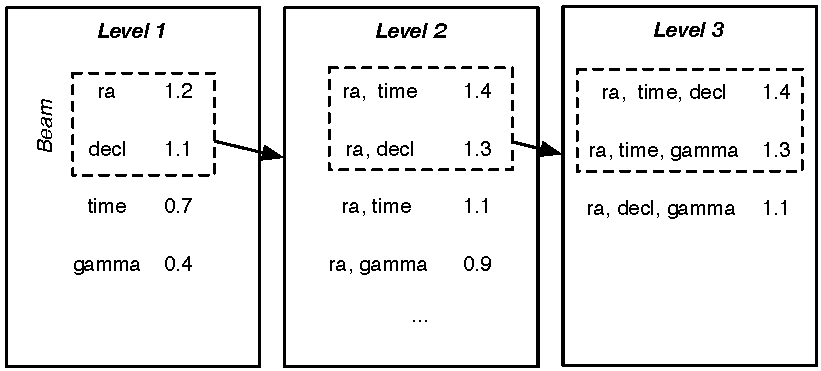
\includegraphics[width=\columnwidth]{images/beam-search}
\caption{Example of Beam Search, with $D=3$ and beam size $B=2$}
\label{pic:beam-search}
\end{figure}
Our algorithm is based on \emph{beam search}, illustrated in
Figure~\ref{pic:beam-search}.  To initialize the algorithm, we compute the
strength of each variable separately. We sort the candidates, and keep the top
$B$ elements. We call this set the \emph{beam}, greyed in the figure. Then, we
generate new candidates, by appending each variable of the database to each
variable in the beam. We obtain views with two columns.  We compute the
strength of these views, keep the top $B$ strongest and discard the others.
This gives us a new beam. We repeat the procedure until the views in the beam
contain $D$ variables, or the views stop improving.
Algorithm~\ref{algo:beam_search} presents the full procedure.

\begin{algorithm}[t]
\caption{Beam Search for view selection}
\label{algo:beam_search}
\begin{algorithmic}
    \Function{TopViews}{$K$, $D$, $B$, $DB$}
    \State $\text{Beam} \gets \{\}$
    \For{$i \in [1, D]$}
        \State $\text{Cand} \gets \{\}, \text{Scores} \gets \{\}$
        \For{$V \in \text{Beam}$}
            \For{$X \in \text{columns}(DB)$}
            \State $\text{Cand} \gets \text{Cand} \cup \{V \cup \{X\} \}$
            \State $\text{Scores} \gets \text{Scores} \cup \sigma(V \cup \{X\}) $
            \EndFor
        \EndFor
        \State $\text{Beam} \gets \text{findTopK}(\text{Cand}, \text{Scores}, B)$
    \EndFor
    \State \Return $\text{findTopK}(\text{Cand}, \text{Scores}, K)$
    \EndFunction
\end{algorithmic}
\end{algorithm}
\begin{figure}[t!]
\centering
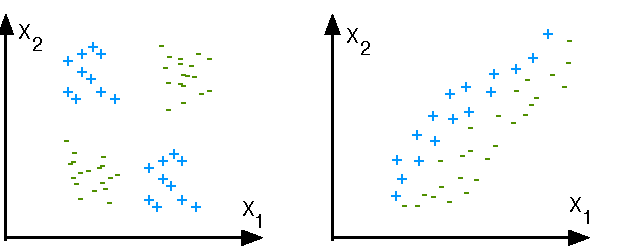
\includegraphics[width=0.7\columnwidth]{images/strength-jump}
\caption{Limit cases of the beam search strategy. The variables $X_1$ and
$X_2$ represent two dimensions. The symbol and color of the plots represent
the value of the target. }
\label{pic:strength-jump}
\end{figure}
Thanks to our strategy, we avoid exploring an exponentially large search
space. Instead, we compute the strengths of at most $N.B$ candidates at each
level. The size of the beam lets us control the trade-off between accuracy and
runtime. With a small beam, we evaluate less candidates, and thus terminate
earlier. Oppositely, a large beam lets us explore more candidates.  Let us
explain why this is necessary. At each level of the algorithm, we discard the
views which are too weak to reach the top $B$ candidates. We assume that if a
combination of column is weak at level $i$, then it will be weak at all
subsequent levels.  Unfortunately, this assumption does \emph{not} hold: we can
form strong views by combining weak columns; there are ``jumps'' in the search
space.  Consider for instance the two classic scenarios pictured in Figure
\ref{pic:strength-jump}.  The dimensions $X_1$ and $X_2$ taken in isolation are
weak: we can infer no useful information about the target from either of them.
However, their combination is very interesting. Equivalently, the views
$\{X_1\}$ and $\{X_2\}$ have a very poor strength, but $\{X_1, X_2\}$ is an
excellent candidate. If the beam is too tight, we may discard $\{X_1\}$ and
$\{X_2\}$ early because they have a low score.  This would be a mistake,
because we lose the opportunity to discover $\{X_1, X_2\}$. Therefore, we
recommend to set $B > K$. During our experiments, we obtained excellent results
with $B \geq 2.K$ (cf.~\ref{sec:exp-view-selection}).

\subsection{Approximations and Refinements}
In total, we evaluate the strength of $B.N$ candidates for the $D$
levels of the beam search. To carry out this computation,  we can either use
the exact formulation of strength, as shown in Equation~\ref{eq:strength}, or
use the approximation scheme presented in Section~\ref{sec:approximate}. In
Claude's implementation, we opted for a hybrid approach. We perform the first
two levels of search with the exact strength (which is equivalent to building
the co-dependency graph).  Then, for all subsequent steps, we use the
approximations. Finally, we revert to the exact strength for the top $k$
ranking, at the very end of the procedure. Thanks to this enhancement, we
obtain significant speed gains at little accuracy cost.

\subsection{Deduplication}
\label{sec:variety}

\begin{figure}[t!]
\centering
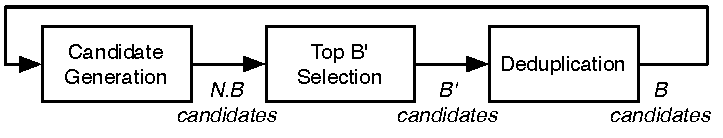
\includegraphics[width=\columnwidth]{images/deduplication}
\caption{Beam search augmented with a deduplication step. We display in italic
the size of the intermediate results. Note that $N.B \geq B' \geq B$.}
\label{pic:deduplication}
\end{figure}
Our algorithm seeks strong views. In some cases however, it may be preferable
to have weaker but more diverse views. To deal with those cases, we introduce
an optional \emph{deduplication} step, during which we reduce the number of
views with an algorithm from the literature. As pictured in
Figure~\ref{pic:deduplication}, we run this procedure at the end of each
beam search iteration.  By definition, deduplication reduces the number
of candidates. Therefore, to obtain $B$ views at the end of the algorithm, we
must generate $B' > B$ views beforehand. A low $B'$ yields more variety,
while a high $B'$ may lead to stronger views.

Authors have proposed quantity of methods to deduplicate itemsets in the
pattern mining literature~\cite{xin2005mining, van2006compression}. We opted
for a simple compression-based approach. First, we compute the dissimilarity
between every pair of views with the Jaccard dissimilarity. Given two views
$V_i$ and $V_j$, it is defined as follows: $d_J(V_i, V_j) = |V_i \cap V_j | / |
V_i \cup V_j |$. We then cluster the resulting matrix with Partitioning Around
Medoids, an algorithm of type k-medoids.  We refer the interested reader to the
literature for more details~\cite{kaufman2009finding}.






\section{Detecting Points Of Interest}
\label{sec:detec}

We previously described how to find strong views. We now
explain how to identify $P$ points of interests for each of these views. 

Fortunately, finding POIs is an instance of a known problem called
\emph{subgroup discovery}~\cite{klosgen1996explora, wrobel1997algorithm}, which
can be formulated as follows: given a set of tuples, a target column and a
measure of exceptionality, detect sets of tuples for which the target behaves
exceptionally. In our case, we instantiate the exceptionality measure
with divergence. 

As pointed our by van Leeuwen and Knobbe~\cite{van2011non}, we can also solve
the subgroup discovery problem with beam search.  Let $V$ represent the view to
analyze. As the variables are binned, can form a grid over $V$, as shown in
Figure~\ref{fig:binningexample}. We denote by $b$ the number of bins for each
variable. To initialize the algorithm, we compute the divergence of each cell
and keep the top $B_{POI}$ most divergent. We obtain our beam. We then ``drill
into'' each of these cells: we decompose them into smaller cells by splitting
the edges into $b$ bins. We evaluate the new candidates and keep the top
$B_{POI}$ most divergent. We reiterate until the algorithm converges.

In practice, KL-based approaches tends to favor smaller regions. Therefore,
Beam Search may converge late, or not at all. A practical solution is to set a
minimum count threshold. Alternatively, we can alter our model to take the size
into account~\cite{van2011non}. Let $R$ represents a region with count $|R|$,
and $|DB|$ represent the number of tuples in the database. We introduce the
\emph{weighted} deviation $\delta_w(R) = |R|/|DB| \times \delta(R)$. This new
score introduces a penalty for small POIs.







\section{Experiments}
\label{sec:experiments}
\begin{table}
    \centering
    \small
    \begin{tabular}{r c c c c} 
        \hline
        Dataset & Columns & Rows & \#Views & \#Variables\\
        \hline
        MuskMolecules & 167 & 6,600 & 22 & 18\\
        Crime & 128 & 1,996 & 20 & 17\\
        BreastCancer & 34 & 234 & 10 & 13\\
        PenDigits & 17 & 7,496 & 9 & 10\\
        BankMarketing & 17 & 45,213 & 11& 8\\
        LetterRecog & 16 & 20,000 & 10 & 12\\
        USCensus & 14 & 32,578 & 10 & 7\\
        MAGICTelescope & 11 & 19,022 & 1 & 10\\
        \hline
    \end{tabular}
    \caption{Characteristics of the datasets. The last two columns are used for
    comparison with 4S, cf. Section~\ref{sec:exp-view-selection}.}
    \label{tab:datasets}
\end{table}
We now present our experimental results. All our experiments are based on 8
datasets from the UCI Repository, described in Table~\ref{tab:datasets}. The
files are freely available online\footnote{archive.ics.uci.edu/ml/}. In several
experiments, we report the \emph{normalized} view strength instead of the usual
strength; if $V$ is a view with entropy $H(V)$, we obtain it as follows:
$\sigma_{norm}(V) = \sigma(V) / H(V)$.

\subsection{Detailed Example: Crimes in the US}
\label{sec:crime}
\begin{table}[t]
  \centering
  \small
  \rowcolors{2}{gray!25}{white}
  \begin{tabulary}{\columnwidth}{L c}
    \hline
    View & Score (normalized)\\
    \hline
    Police.Overtime, Pct.Vacant.Boarded, Pct.Race.White & 0.51\\
    Pct.Families.2.Parents, Pct.Race.White, Police.Requests.Per.Officer & 0.49\\
    Pct.Police.White, Pct.Police.Minority, Pct.Vacant.House.Boarded& 0.37\\
    Pct.Empl.Profes.Services, Pct.Empl.Manual, Pct.Police.On.Patrol & 0.37\\
    Pct.Retired, Pct.Use.Public.Transports, Pct.Police.On.Patrol& 0.35 \\
    Pct.Recently.Moved, Population.Density, Police.Cars & 0.34 \\
    \hline
\end{tabulary}
    \caption{Example of views generated by Claude for the US Crime dataset.}
    \label{tab:crime_views}
\end{table}
\begin{figure}[t!]
    \centering
    \begin{subfigure}[b]{0.45\columnwidth}
    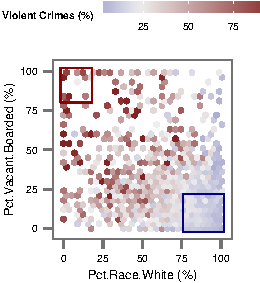
\includegraphics[width=\textwidth]{plots/crime1}
    \end{subfigure}
    \begin{subfigure}[b]{0.45\columnwidth}
    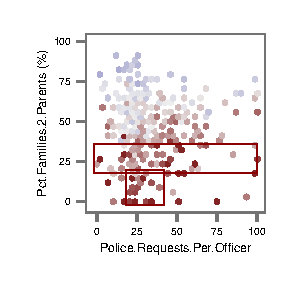
\includegraphics[width=\textwidth]{plots/crime2}
    \end{subfigure}

    \begin{subfigure}[b]{0.45\columnwidth}
    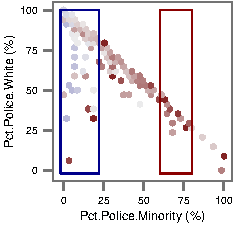
\includegraphics[width=\textwidth]{plots/crime3}
    \end{subfigure}
    \begin{subfigure}[b]{0.45\columnwidth}
    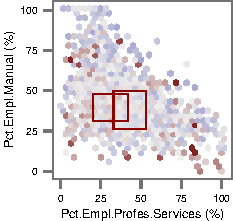
\includegraphics[width=\textwidth]{plots/crime4}
    \end{subfigure}
    
    \begin{subfigure}[b]{0.45\columnwidth}
    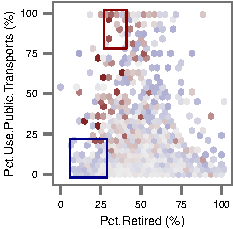
\includegraphics[width=\textwidth]{plots/crime5}
    \end{subfigure}
    \begin{subfigure}[b]{0.45\columnwidth}
    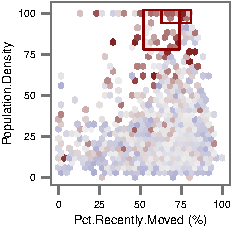
\includegraphics[width=\textwidth]{plots/crime6}
    \end{subfigure}
\caption{Heatmaps of the US Crime Dataset, based on Claude's output. Each box
represents a Point of Interest.}
\label{pic:crime_charts}
\end{figure}

In this section, we showcase Claude with a real-life example: we analyze the
Communities and Crime dataset form the UCI
repository\footnote{archive.ics.uci.edu/ml/datasets/Communities+and+Crime}.
Our aim is to understand which US cities are subject to violent crimes. Our
database compiles crime data and socio-economic indicators about 1994
communities, with a total of 128 variables. The data comes mostly from the
90's, and it was provided by official US sources - among others, the 1990 US
census and the 1995 FBI Uniform Crime Report. All the variables are normalized
to have a minimum of 0 and a maximum of 100.

We generated $K=100$ views with up to $D=3$ dimensions, both with and
without deduplication. We present a selection of views in
Table~\ref{tab:crime_views}, along with 2-dimension heat maps in
Figure~\ref{pic:crime_charts}. Observe that strong views have a visual
signature: in the top two maps, the blue and red areas are neatly separated. In
the bottom two views, the distinction is less clear.

The first view of Table \ref{tab:crime_views} is the best one we found:
\texttt{Police. Overtime, Pct.Race.White, Pct.Vacant.Boarded}. It has a score
of 0.51. which means that these three variables contain 51\% of the target's
information. The columns \texttt{Police. Overtime} and \texttt{Pct.White.Race}
respectively describe the average time overworked by the police and the
percentage of caucasian population. The third variable,
\texttt{Pct.Vacant.Boarded} was surprising to us: it describes the
percentage of vacant houses which are boarded up.  How does this relate to
crime? We could assume that boarded houses are associated with long term
abandon, and thus, poverty. The top-left plot of Figure \ref{pic:crime_charts}
shows the relation between race, boarded houses and crime. Observe that the
variables complement each other: a high proportion of caucasians may or may not
lead to low crime. However, a high proportion of caucasians \emph{combined
with} a low rate of boarded house correspond to safe areas, while little
caucasians and many boarded houses correspond to more violent communities.

Our second view shows that cities with more monoparental families tend to be
more violent: the correlation is clearly visible, and both POIs point to the
bottom of the chart. However, close inspection also reveals surprises: a few
communities have a relatively high number of two-parents families, but also
high indicators of police requests and crime (in the top right corner of the
chart). Manual queries reveals that many of these cities are located in the
suburbs of Los Angeles, and contain a majority of Hispanics. Does this explain
the peculiarity? We leave this question open for future investigations. We see
that some findings come from the recommendations directly while others are
serendipitous.  But in both cases, Claude lets us discover ``nuggets'' with
little prior knowledge and few assumptions. 

\subsection{View Strength and Prediction}
\label{sec:view-strengh}
\begin{figure}[t!]
\centering
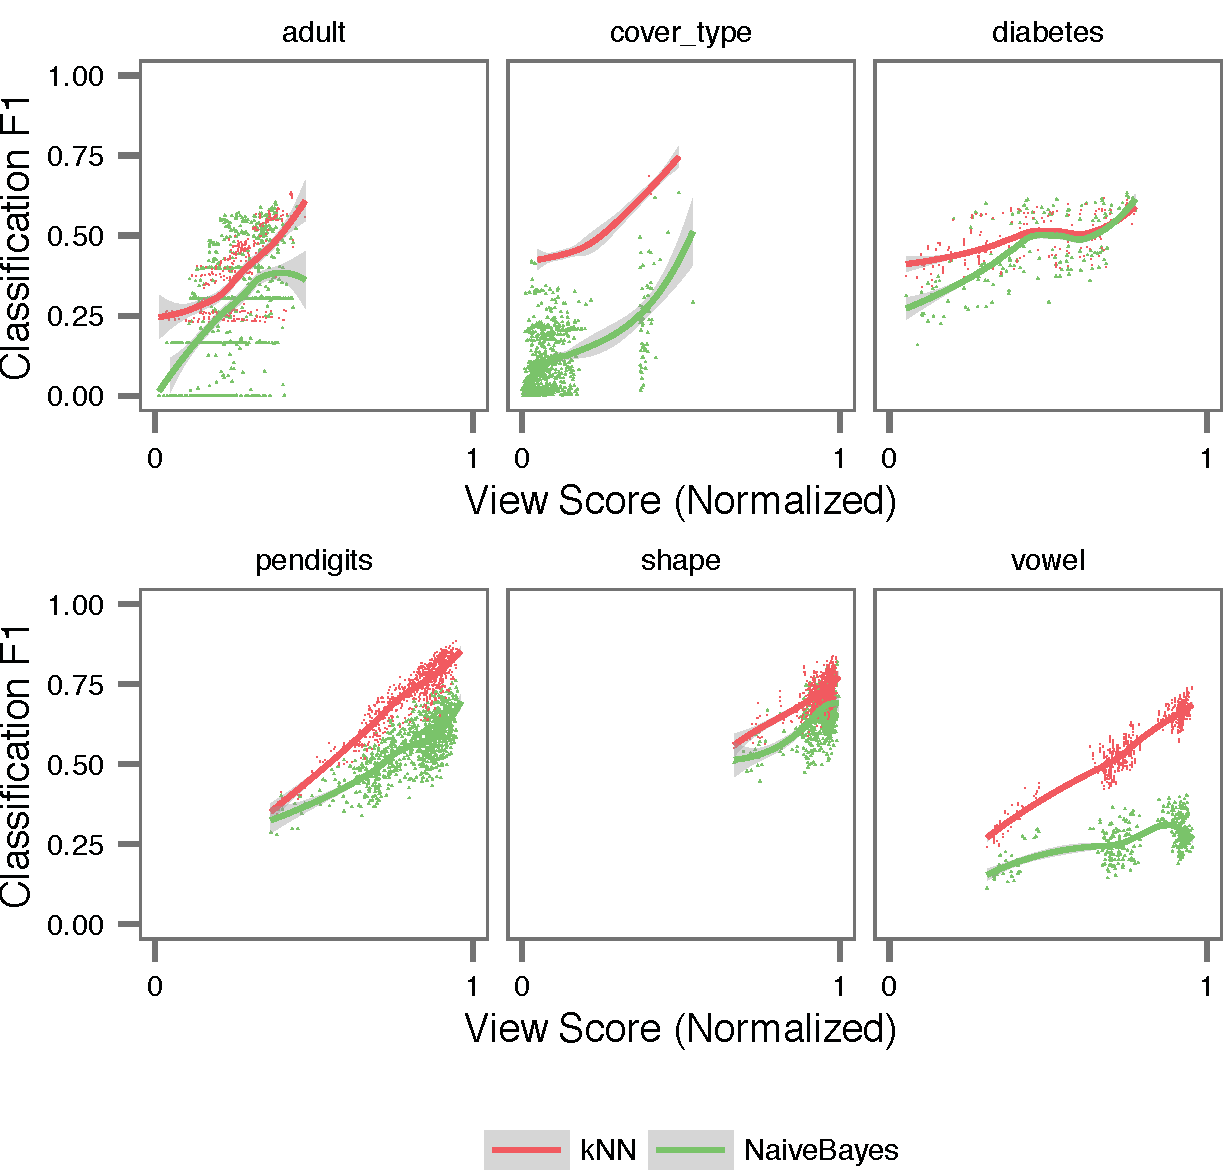
\includegraphics[width=\columnwidth]{plots/compare-strength-f1}
\caption{Strength vs. Classification accuracy for 500 random views. We obtained
    the blue and red lines with simple linear regression.}
\label{pic:strength-vs-f1}
\end{figure}
In this section, we show experimentally that our notion of view strength
``works'', e.g. that strong views effectively provide information about the
target column. To verify this assumption, we simulate users with statistical
classifiers. Consider a view $V$ over a database. If a classifier can predict
the value of the target from $V$'s columns, then $V$ is informative.
Oppositely, if the classifier fails, then $V$ is potentially uninteresting. In
a nutshell, we should observe a positive correlation between views strength
and classification accuracy.

We now detail our experiment. We chose three datasets from the UCI repository.
For each dataset, we generated 500 random views and measured their strengths.
We then trained classifiers on each of these views, and measured their
performance. We report the results in Figure \ref{pic:strength-vs-f1}. We chose
two classification algorithms: Naive Bayes, and 5-Nearest Neighbors.  We chose
those because they contain no built-in mechanism to filter out irrelevant
variables (as opposed to, e.g., decision trees). We measure classification
performance with 5-fold validation, to avoid the effects of overfitting.

In all three cases, we observe a positive correlation between the strengths of
the views and the accuracy of the predictions. We confirm these observations
with statistical tests: the coefficients of determination ($R^2$) vary between
0.11 and 0.84, which indicates the presence of a trend (despite some
variability). Furthermore, the p-values associated to the coefficients are all
under $10^{-3}$, this gives us excellent confidence that the strength
influences positively the prediction accuracy. In conclusion, strong views are
indeed more instructive.


\subsection{View Selection}
\label{sec:exp-view-selection} 

We now evaluate Claude's output and runtime in detail. In this section, we
verify if Claude's algorithm produces good views in a short amount of time. To
do so, we compare it to four methods, three of which come from the machine
learning literature.  Our first baseline, \texttt{Exact}, is similar to
Claude, but we removed the approximation scheme presented in
\ref{sec:approximate} - instead we compute the exact the mutual information, as
in Equation~\ref{eq:strength} The method should be slower, but more accurate. 

The second algorithm, \texttt{Clique}, is a top-down approach inspired by
recent work on pattern mining~\cite{xie2010max}. We build a graph where each
vertex $i$ represents a column $D_i$, and each edge $(i,j)$ represents the view
$\{D_i, D_j\}$. We then eliminate all the edges except those which represent
the top $B$ views. To detect views with $D>2$ columns, we seek cliques in this
degenerated graph. We used the \texttt{igraph} package from R. We expect this
algorithm to be very fast, but less accurate.

The third method, \texttt{Wrap 5-NN}, is a classic feature selection
algorithm~\cite{guyon2003introduction}. The idea is to train a 5-Nearest
Neighbor classifier with increasingly large sets of variables. We first test
each variable separately, and keep the column which led to the best prediction.
Then we keep adding variables in a breadth-first manner, until the
quality of the predictions stops increasing or we reach $n$ variables. Our
implementation is based on the \texttt{class} package from R.  We modified the
original algorithm to maintain and update $q$ distinct sets of variables
instead of just one. We chose the nearest neighbor algorithm because it is
fast, and it gave us good performance, as shown in \ref{sec:view-strengh}. We
expect this algorithm to be very slow, but close to optimal.

Finally, the last method, \texttt{4S} is a state-of-the-art subspace search
method from the unsupervised learning literature~\cite{nguyen20134s}. The aim
of the algorithm is to detect ``interesting'' subspaces in large databases,
independently of a target variable. To do so, it seeks groups of variables
which are mutually correlated, with sketches and graph-based techniques.  We
used the author's implementation, written in Java. We expect the algorithm to
be very fast and reasonably accurate.

We use 8 public datasets, presented in Section \ref{sec:experiments}. For a
fair comparison, we must ensure that each algorithm generates the same number
of views ($K$) with the same number of variables ($D$).  However, we have no
way to specify these parameters a priori with 4S, because the algorithm has a
built-in mechanism to pick optimal values. Therefore, we run 4S first on each
dataset, we let it chose $K$ and $D$, and we use these values for the remaining
algorithms.  We report the obtained parameters in Table~\ref{tab:datasets}.

We implemented Claude in R, except for some information theory primitives
written in C. For practical reasons, we interrupted all the experiments which
lasted more than 1 hour. Our test system is based on a 3.40 GHz Intel(R)
Core(TM) i7-2600 processor. It is equipped with 16 GB RAM, but the Java heap
space is limited to 8 GB. The operating system is Fedora 16. 

\begin{figure*}[t!]
\centering
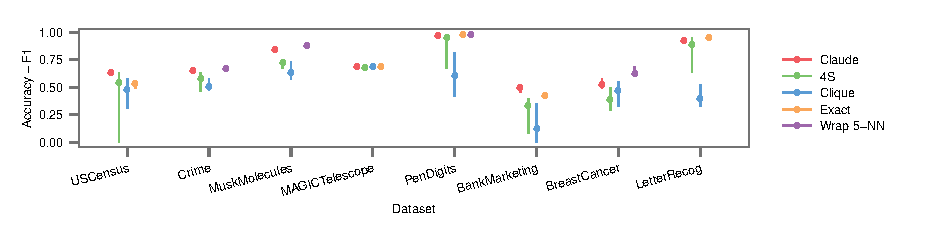
\includegraphics[width=1.8\columnwidth]{plots/view-scores}
\caption{Performance of the View Selection algorithms. For each data set, we
    generate $q$ views, train a 5-NN classifier over the columns of each view
    and report the classification accuracy (F1, 5-fold cross validation). The
    points represent median scores, the bars represent the lowest and greatest
    scores.} 
\label{pic:column-select-score}
\end{figure*}
\begin{figure*}[t!]
\centering
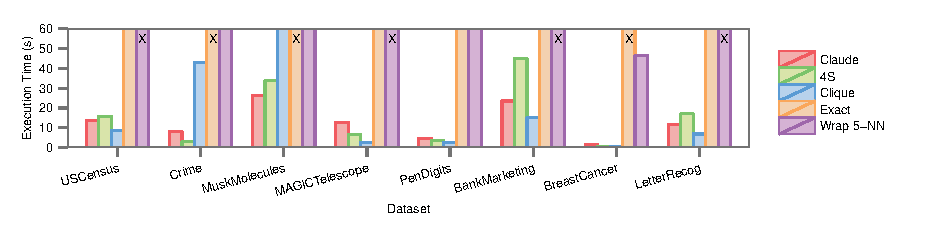
\includegraphics[width=1.8\columnwidth]{plots/view-times}
\caption{Execution time of the View Selection algorithms. A \texttt{X} symbol
indicates that the experiment did not finish within 3,600 seconds.}
\label{pic:column-select-time}
\end{figure*}

\textbf{Accuracy.} In Figure \ref{pic:column-select-score}, we compare the
quality of the views returned by each algorithm. For each competitor, we
generate $q$ views with $n$ variables, train a classifier on each view and
measure the quality of the predictions. For the classification, we use both
Naive Bayes and 5-Nearest Neighbors, and report the highest score.  We measure
accuracy with the F1 score on 5-fold cross validation; higher is better.

The method \texttt{Wrap 5-NN} comes first for all the datasets on which it
completed. This is not surprising since the algorithm optimizes exactly what we
measure: \texttt{Wrap 5-NN} is our ``gold standard''. Our two algorithms,
\texttt{Claude} and \texttt{Exhaustive}, come very close. This indicates that
both algorithms find good views, and that our approximation scheme works
correctly.  The algorithms \texttt{4S} and \texttt{Clique} come much lower. As
\texttt{4S} is completely unsupervised, we cannot expect it to perform as well
as the other approaches. The assumptions behind \texttt{Clique} are
apparently too naive.

\textbf{Runtime.} Figure~\ref{pic:column-select-time} shows the runtime of our
experiments. The algorithms \texttt{Exact} and \texttt{Wrap 5-NN} are orders of
magnitude slower than the other approaches. The remaining three approaches are
comparable: depending on the datasets, either \texttt{Clique} or \texttt{4S}
come first. Claude comes first for \texttt{MuskMolecules}, and close
second for all the other datasets. We conclude that Claude is compairable to
its competitors in terms of runtime, but it generates better views.

\begin{figure}[t!]
\centering
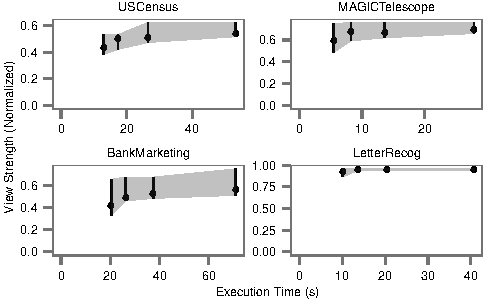
\includegraphics[width=\columnwidth]{plots/view-vary-beam}
\caption{Impact of the beam size on the execution time and view strength. For
each dataset, we generated 25 views with beam size 25, 50, 100 and 250. The
points represent the medium scores, the bars represent the lowest and greatest
scores.}
\label{pic:view-beam}
\end{figure}
\begin{figure}[t!]
\centering
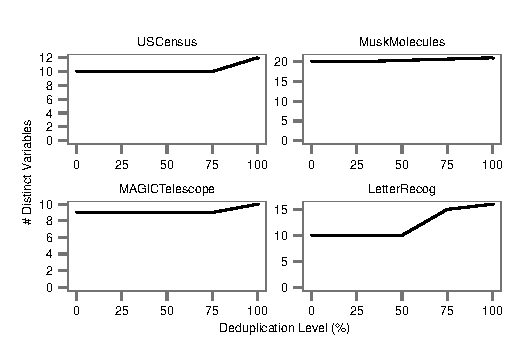
\includegraphics[width=\columnwidth]{plots/view-vary-diversification}
\caption{Impact of the deduplication. We generated 25 views for each dataset.
The y-axis presents the average Jaccard dissimilarity between every pair of
views.}
\label{pic:view-diversification}
\end{figure}
\textbf{Impact of the beam size.} Figure~\ref{pic:view-beam} shows the impact
of the beam size $B$ on Claude's performance, for 4 databases. To obtain these
plots, we ran Claude with $K=25$ and $D=5$, and varied $B$ between 25 and 250.
We observe that smaller beams lead to lower execution times, while larger beam
lead to stronger views. However, the heuristic converges fast: we observe
little to no improvement for $B$ greater than 50.

\textbf{Impact of the deduplication.} We show the impact of our deduplication
strategy in Figure \ref{pic:view-diversification}.  We ran Claude with $K=25$
and $D=5$ and increased the level of deduplication, i.e., varied the value of
$B'$ between $B$ and $N.B$ (cf. Section \ref{sec:variety}). A level of 0\%
means that $B'=B$. A level of 100\% means that $B'=N.B$. To measure the
diversity of the views, we measured the Jaccard dissimilarity between every
pair of views and averaged the results. We observe that the strategy works in
all four cases, but with different levels of efficiency. In the
\texttt{BankMarketing} case, our strategy almost doubles the pairwise
dissimilarity of the views. The effect is much lighter on datasets with few
columns, such as \texttt{USCensus} and \texttt{MAGICTelescope}.
\begin{figure*}[t!]
\centering
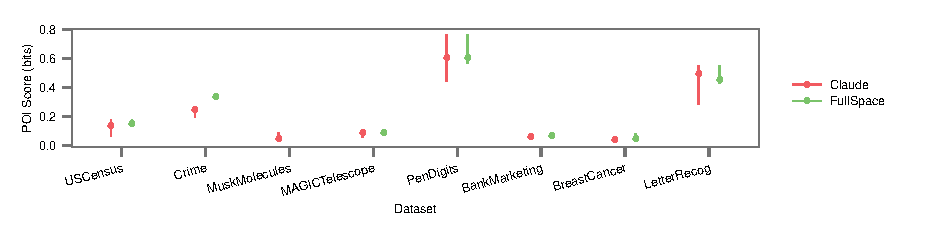
\includegraphics[width=1.8\columnwidth]{plots/POI-score}
\caption{Quality of the Point of Interests. For each view, we detect $P=10$
POIs. The
    points represent median scores, the bars represent the lowest and greatest
    scores.}
\label{pic:POI-quali}
\end{figure*}
\begin{figure*}[t!]
\centering
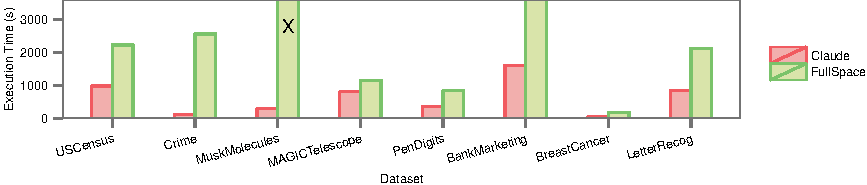
\includegraphics[width=1.8\columnwidth]{plots/POI-timing}
\caption{Execution time of the POI detection. A \texttt{X} symbol
indicates that the experiment did not finish within 7,200 seconds.}
\label{pic:POI-time}
\end{figure*}

\subsection{POI Detection}
\label{sec:exp-poi}

In this section, we evaluate Claude's POI detection strategy. We compare two
approaches. The first approach is the algorithm presented in the paper: first
we search $K$ views, then we return $P$ POIs per view. The second approach,
\texttt{FullSpace}, is the method used in much of the recent Subgroup Discovery
literature \cite{van2011non, duivesteijn2010subgroup}.  The idea is to apply
Beam Search on the whole database directly. Instead of seeking $P$ POIs in $K$
projections, we seek $K.P$ selections from the full column space; we skip the
view selection step. We use the same datasets as previously. Our default
parameters are $K=25$, $D=5$, $B=50$ and $P=10$. To set the beam size, we use a
rule of thumb: $B_{POI} = 2.k$ ($B_{POI}$ is the beam used for POI detection,
not for view search). To gather sufficient data, we raise our time limit to 2
hours. 

Figure \ref{pic:POI-quali} compares the quality of the POIs found by both
algorithms. The strategy \texttt{FullSpace} gives slightly better results on
\texttt{Crime} and \texttt{PenDigits}, but the difference is close to null. The
scores are similar on all the other datasets. We conclude that Claude's POIs
are very close to those found by a state-of-the-art Subgroup Discovery
approach.  Figure~\ref{pic:POI-time} compares the runtimes of both approaches.
We observe that Claude is much faster than \texttt{FullSpace}. The difference
grows with the number of columns: the runtimes are almost similar for datasets
with few columns (\texttt{MAGICTelescope}), but \texttt{Claude} is considerably
faster for larger databases (more than an order of magnitude difference for
\texttt{MuskMolecules}). This is a positive side-effect of our approach:
decoupling view search and POI extraction allows us to find subgroups faster in
high dimension datasets.

\section{Related Work}
\label{sec:related}

\textbf{SQL Query Recommendation.} We identify two types of approaches:
\emph{human-driven} systems and \emph{data-driven} systems. Human-driven
systems learn from user feedback. For instance, Chatzopoulou et al.  make
recommendations from query logs, similarly to search engines
\cite{chatzopoulou2009query}. In Explore-by-Example, the system infers queries
from examples provided by the user \cite{dimitriadou2014explore}. With Charles,
the engine decomposes user queries into smaller queries, which can then be
decomposed further \cite{sellam2013meet}.  Sarawagi's method builds a maximum
entropy model over the database from the user's history
\cite{sarawagi2000user}. Bonifati et al. propose a similar method to recommend
joins \cite{bonifati2014interactive}.  Claude competes with neither of these
approaches, since it uses the content of the database only.

Our work is closer data-driven data recommendation. The general idea is to
build a statistical model of the database, and find regions which behave
unexpectedly. Sarawagi et al. have published seminal work on this
topic~\cite{sarawagi1998discovery}. Their system requires that the data is
organized in an OLAP cube (with hierarchical dimensions), it supposes that the
users know which variables to use, and it seeks thin-grained deviations.
Oppositely, our system uses regular tables, it recommends views (not only
selections) and it seeks large trends. Similarly, constrained gradient
analysis~\cite{imielinski2002cubegrades, dong2001mining} focuses only on
hierarchical data cubes. More recently, Dash et al. have proposed a method to
reveal surprising subsets in a faceted search context \cite{dash2008dynamic}.
This method is related to Claude, but it targets document search, it does not
recommend views.

\textbf{Projection Search.} Authors from the data visualization literature have
proposed methods to detect the ``best'' projections of multidimensional data
sets, such as Projection Pursuit~\cite{yoi1974projection},
Scagnostics~\cite{wilkinson2005graph}, or Tatu et al.'s relevance
measures~\cite{tatu2011automated}. Such methods would form excellent complements
for Claude's recommendations. Nevertheless, most of them focus on 2-dimensional
scatterplots, are limited to continuous variables, and involve materializing
and analyzing every possible 2D projection of the data.

\textbf{Feature Selection, Subspace Search.} Choosing which variables to use for
classification or regression is a crucial problem, for which dozens of methods
were proposed \cite{guyon2003introduction}. Similarly to Claude, some of these
methods rely on mutual information~\cite{peng2005feature}. Nevertheless, the
objective is different. A feature selection algorithm seeks \emph{one} set of
variables, on which a statistical predictor will perform optimally. Claude seeks
several, small sets of variables, simple enough to be interpreted by a humans.
In fact, Claude is halfway between inference and exploration.
On the unsupervised learning side, our work is close to subspace search. The
idea is detect subspaces where the data is clustered distinctly
\cite{keller2012hics,nguyen20134s}. We compare Claude to state-of-the-art
methods in our Experiments section.

\section{Conclusion}
\label{sec:conclusion}
We formalized what makes a query ``interesting'', using the mutual information
and the Kullback-Leibler divergence. We presented practical methods to detect
these queries, using carefully designed approximations.  Finally, we presented
and evaluated Claude, a system based on these ideas. The methods we developed
for this study have broader applications than the strict realm of query
recommendation. Our column selection scheme competes with state-of-the-art
feature selection methods. Also, the idea to decouple column selection
selection from subgroup search could benefit a wide range of subgroup discovery
algorithms.

We are genuinely excited about the possible extensions of this study. Future
work includes dealing explicitly with the structure of the data, e.g.,
hierarchical dimensions and relational joins. We will study how to integrate
Claude more tightly with visualizations, for a fully interactive experience.
Finally, we will refine our framework with causation models.
